% Created 2022-02-18 Fr 10:31
% Intended LaTeX compiler: pdflatex
\documentclass[presentation]{beamer}
\usepackage[utf8]{inputenc}
\usepackage[T1]{fontenc}
\usepackage{graphicx}
\usepackage{grffile}
\usepackage{longtable}
\usepackage{wrapfig}
\usepackage{rotating}
\usepackage[normalem]{ulem}
\usepackage{amsmath}
\usepackage{textcomp}
\usepackage{amssymb}
\usepackage{capt-of}
\usepackage{hyperref}
\usepackage{minted}
\usepackage[utf8]{inputenc}
\usepackage{color}
\usetheme[height=7mm]{Rochester}
\setbeamertemplate{footline}[frame number]
\usecolortheme[accent=red, light]{solarized}
\setbeamercolor{frametitle}{bg=solarizedRebase02,fg=solarizedAccent}
\setbeamercolor{author in head/foot}{bg=solarizedRebase02,fg=solarizedRebase01}
\setbeamercolor{title in head/foot}{bg=solarizedRebase02,fg=solarizedRebase01}
\setbeamercolor{block title}{bg=solarizedRebase0,fg=solarizedRebase02}
\setbeamercolor{block body}{bg=solarizedRebase02,fg=solarizedRebase0}
\setbeamercolor{item}{bg=solarizedRebase02,fg=solarizedAccent}
\beamertemplatenavigationsymbolsempty
\usemintedstyle{manni}
\AtBeginSection[]{
\begin{frame}
\vfill
\centering
\begin{beamercolorbox}[sep=8pt,center,shadow=true,rounded=true]{title}
\Huge\insertsectionhead\par%
\end{beamercolorbox}
\vfill
\end{frame}
}
\usetheme{default}
\author{Thomas Hausberger, Matthias Panny \\ Ursprünglich erstellt von Sebastian Stabinger}
\date{SS2022}
\title{Zeiger, Referenzen, das Slicing Problem und Polymorphismus}
\hypersetup{
 pdfauthor={Thomas Hausberger, Matthias Panny \\ Ursprünglich erstellt von Sebastian Stabinger},
 pdftitle={Zeiger, Referenzen, das Slicing Problem und Polymorphismus},
 pdfkeywords={},
 pdfsubject={},
 pdfcreator={Emacs 27.2 (Org mode 9.4.4)}, 
 pdflang={Ger}}
\begin{document}

\maketitle

\section{Zeiger}
\label{sec:orgd1fe54c}
\begin{frame}[label={sec:orgfdfe725}]{Zeiger in C}
\begin{itemize}
\item Zeiger sind Variablen welche Adressen speichern können (also
normalerweise 64bit Integer)
\item Zeiger haben einen Typ
\begin{itemize}
\item Der Typ eines Zeigers gibt an, was an der Adresse auf die gezeigt
wird gespeichert ist.
\item Im Zeiger selbst wird unabhängig vom Typ immer das gleiche
gespeichert (eine Adresse)
\end{itemize}
\end{itemize}
\begin{center}
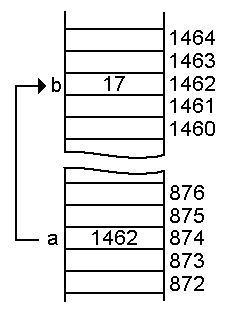
\includegraphics[width=0.3\textwidth]{img/pointer.png}
\end{center}
\end{frame}
\begin{frame}[label={sec:orgf82d720},fragile]{Beispiel und Probleme}
 \begin{block}{Beispiel}
\begin{minted}[numberblanklines=false,fontsize=\scriptsize]{c++}
int intVar = 10;
int *intPtr = &intVar;
cout << intVar << endl;
cout << *intPtr << endl;
intVar = 20;
cout << *intPtr << endl;
\end{minted}
\end{block}
\begin{block}{Probleme}
\begin{minted}[numberblanklines=false,fontsize=\scriptsize]{c++}
int *intPtr2;
// zufaelliger speicherzugriff (pointer wird nicht initialisiert)
cout << *intPtr2 << endl;
int *intPtr3 = NULL;
// zugriff auf speicheradresse 0 (ueblicherweise segmentation fault)
cout << *intPtr3 << endl;
\end{minted}
\end{block}
\end{frame}
\begin{frame}[label={sec:org9bd9d8e},fragile]{Probleme mit Zeigern}
 \begin{block}{Probleme}
\begin{enumerate}
\item Ein Zeiger muss nicht auf ein gültiges Objekt im Speicher zeigen
\item Ein Zeiger kann auch auf nichts zeigen (wenn {\color{solarizedYellow}\verb!NULL!} als Adresse
gespeichert ist)
\item Die Syntax von Zeigern ist am Anfang verwirrend ({\color{solarizedYellow}\verb!*!}, {\color{solarizedYellow}\verb!&!}, \ldots{})
\end{enumerate}
\end{block}
\begin{block}{Vorteile}
Nachdem Zeiger ein sehr einfaches Konzept sind (eine Variable welche
eine Adresse speichert) ist es auch ein extrem mächtiges Werkzeug
\end{block}
\end{frame}
\section{Referenzen}
\label{sec:orgb08a8a5}
\begin{frame}[label={sec:org05eda9c}]{Eigenschaften}
Referenzen verweisen wie Zeiger auf Objekte im Speicher
\begin{block}{Vorteile von Referenzen}
\begin{itemize}
\item Referenzen lösen einige der Probleme mit Pointern
\item Typprüfung des Compilers kann nicht mehr so leicht übergangen werden
\item Referenzen können wie normale Variablen verwendet werden
\end{itemize}
\end{block}
\begin{block}{Nachteile von Referenzen}
\begin{itemize}
\item Referenzen sind weniger flexibel als Zeiger
\begin{itemize}
\item Keine Zeigerarithmetik
\item Keine Möglichkeit direkt auf die Adresse zuzugreifen
\end{itemize}
\end{itemize}
\end{block}
\end{frame}
\begin{frame}[label={sec:org058c988},fragile]{Referenzen --- Syntax}
 \begin{itemize}
\item Um eine Referenz zu erzeugen stellt man ein {\color{solarizedYellow}\verb!&!} an den Anfang eines
Variablen- oder Parameternamens (Äquivalent zu dem {\color{solarizedYellow}\verb!*!} bei einem
Zeiger)
\item \alert{Bei Variablen muss zudem in der gleichen Zeile eine Referenz auf
eine andere Variable zugewiesen werden!}
\item Um eine Referenz auf eine Variable zeigen zu lassen muss nicht wie
bei Zeigern zuerst die Variable mittels {\color{solarizedYellow}\verb!&!} referenziert werden
\end{itemize}
\begin{minted}[numberblanklines=false,fontsize=\scriptsize]{c++}
int x = 23;
int &foo = x;
// foo ist jetzt eine Referenz auf x 
// (foo und x enthalten immer den gleichen Wert)
\end{minted}
\begin{itemize}
\item Auf eine Referenz wird genauso zugegriffen wie auf eine gewöhnliche
Variable (es ist kein Dereferenzieren mit einem {\color{solarizedYellow}\verb!*!} notwendig wie
bei einem Zeiger)
\end{itemize}
\begin{minted}[numberblanklines=false,fontsize=\scriptsize]{c++}
foo = 42;
std::cout << foo << " " << x << std::endl;
\end{minted}
\end{frame}
\begin{frame}[label={sec:org9038e77}]{Referenzen --- Graphische Visualisierung}
\begin{center}
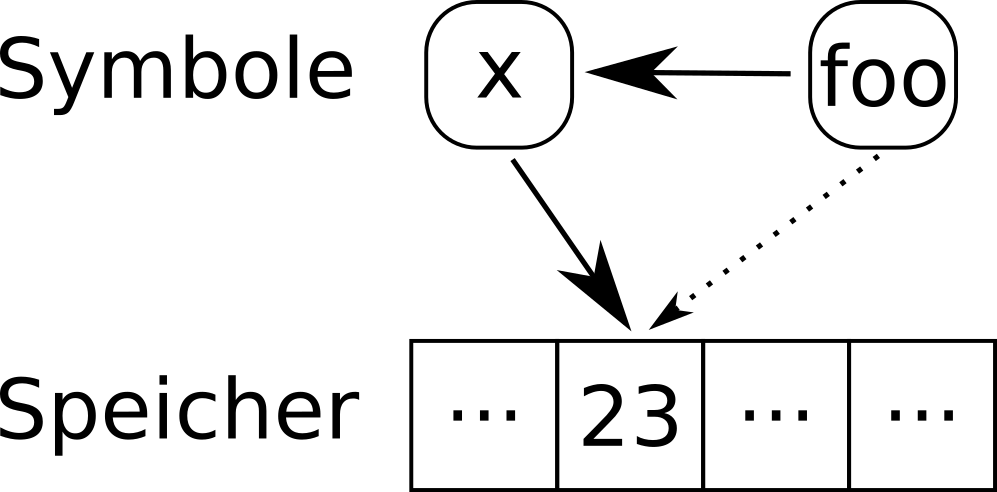
\includegraphics[width=.9\linewidth]{img/references.png}
\end{center}
\end{frame}
\begin{frame}[label={sec:org5fe8625},fragile]{Vergleich zwischen Zeiger und Referenz}
 \begin{minted}[numberblanklines=false,fontsize=\scriptsize]{c++}
// Erzeugen von Variable, Zeiger und Referenz
int intVar = 10;
int *intPtr = &intVar;
int &intRef = intVar;
// Auslesen von Variable, Zeiger und Referenz
cout << intVar << endl;
cout << *intPtr << endl;
cout << intRef << endl;
// Zuweisen an Variable, Zeiger und Referenz
intVar = 20;
*intPtr = 30;
intRef = 40;

cout << intVar << endl; // Ausgabe = 40
\end{minted}

Man sieht also, dass sich Referenzen genauso verwenden lassen wie
Variablen, aber zu großen Teilen die Funktionalität eines Zeigers
haben
\end{frame}
\begin{frame}[label={sec:org4d579f2}]{Referenzen als Parameter}
\begin{itemize}
\item Referenzen als Variablen in "normalem" Code sind eher unüblich
\item Referenzen werden am häufigsten bei Parametern von Funktionen
verwendet:
\begin{itemize}
\item Die übergebenen Parameter müssen dadurch nicht kopiert werden was
gerade bei großen Klassen schneller ist
\item Innerhalb der Funktion können Änderungen an den Parametern
vorgenommen werden welche auch ausserhalb der Funktion sichtbar
sind. Normalerweise funktioniert das nicht, weil die Änderungen
nur an einer Kopie vorgenommen werden.
\end{itemize}
\end{itemize}
\end{frame}
\begin{frame}[label={sec:org7676784},fragile]{Swap mit normalen Parametern, Zeigern, Referenzen}
 \begin{block}{Normale Parameter}
\begin{minted}[numberblanklines=false,fontsize=\scriptsize]{c++}
void swap(int p1, int p2) {
  int temp = p1; p1 = p2; p2 = temp;
}
int a = 2, b = 3; swap(a, b);   // Verwendung
\end{minted}
\footnotesize
Sieht einfach aus, funktioniert aber auch einfach nicht \ldots{}
\end{block}
\begin{block}{Zeiger}
\begin{minted}[numberblanklines=false,fontsize=\scriptsize]{c++}
void swap(int *p1, int *p2) {
    int temp = *p1; *p1 = *p2; *p2 = temp;
}
int a = 2, b = 3; swap(&a, &b); // Verwendung
\end{minted}
\end{block}
\begin{block}{Referenzen}
\begin{minted}[numberblanklines=false,fontsize=\scriptsize]{c++}
void swap(int &p1, int &p2) {
  int temp = p1; p1 = p2; p2 = temp;
}
int a = 2, b = 3; swap(a, b);  // Verwendung
\end{minted}
\end{block}
\end{frame}
\begin{frame}[label={sec:org6c3d990}]{Swap -- Graphische Visualisierung}
\begin{center}
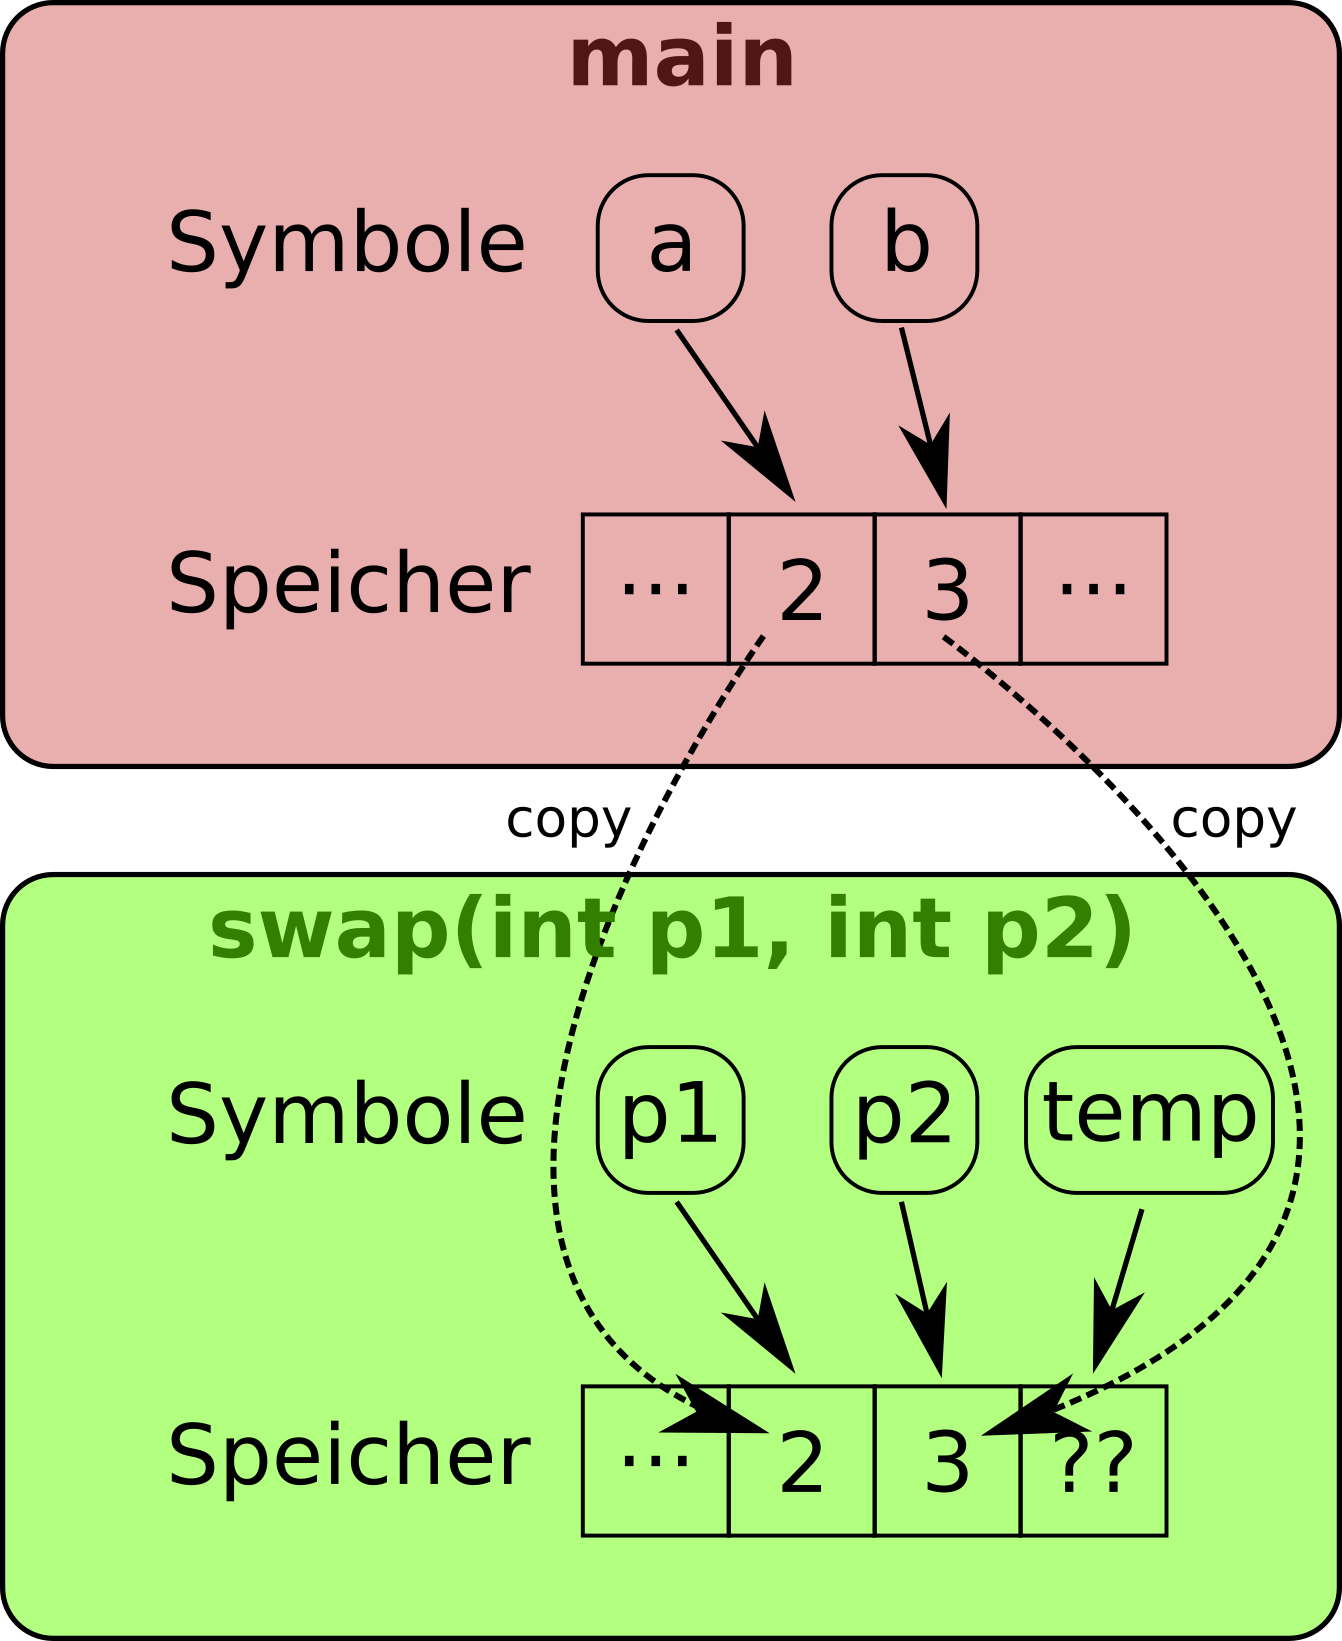
\includegraphics[width=0.6\textwidth]{img/swap_copy.png}
\end{center}
\end{frame}
\begin{frame}[label={sec:org03f5846}]{Swap -- Graphische Visualisierung}
\begin{center}
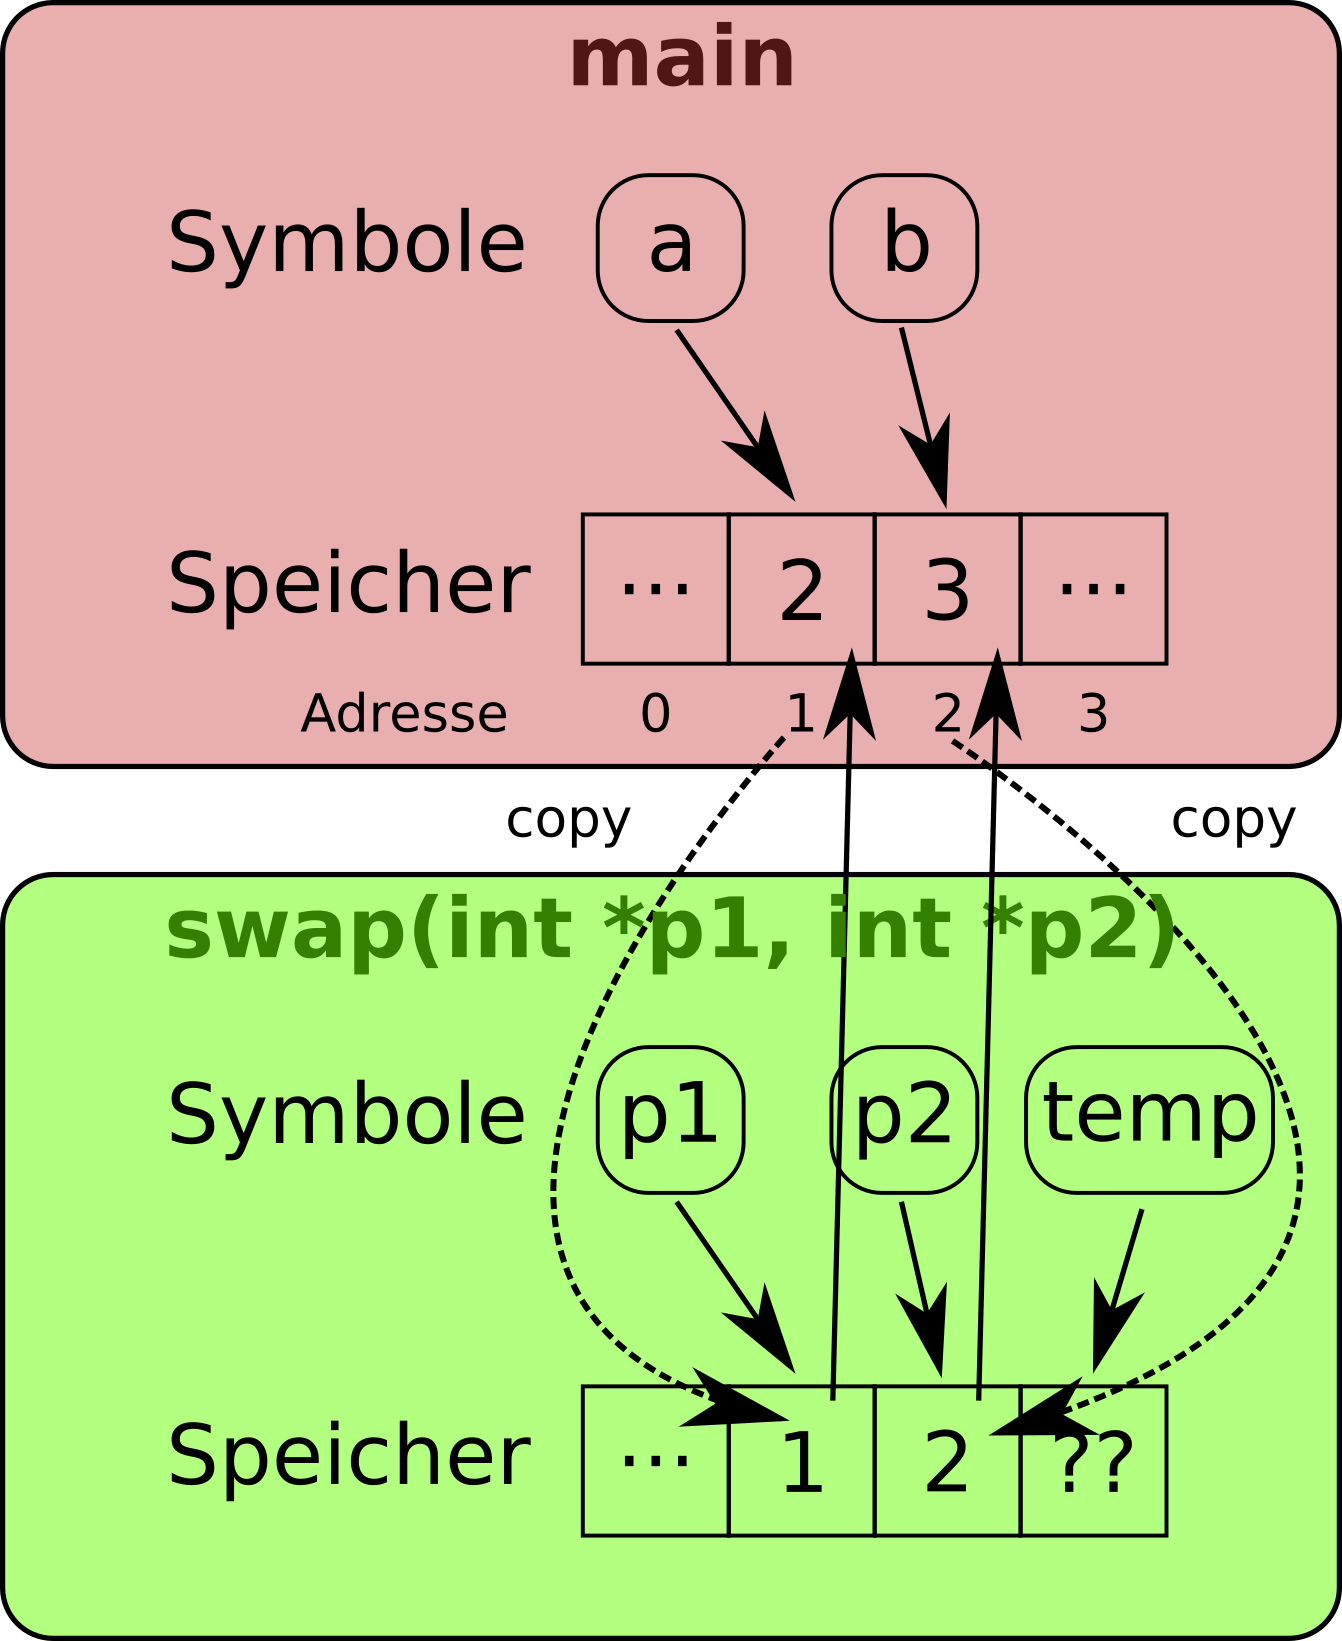
\includegraphics[width=0.6\textwidth]{img/swap_point.png}
\end{center}
\end{frame}
\begin{frame}[label={sec:orge1390b5}]{Swap -- Graphische Visualisierung}
\begin{center}
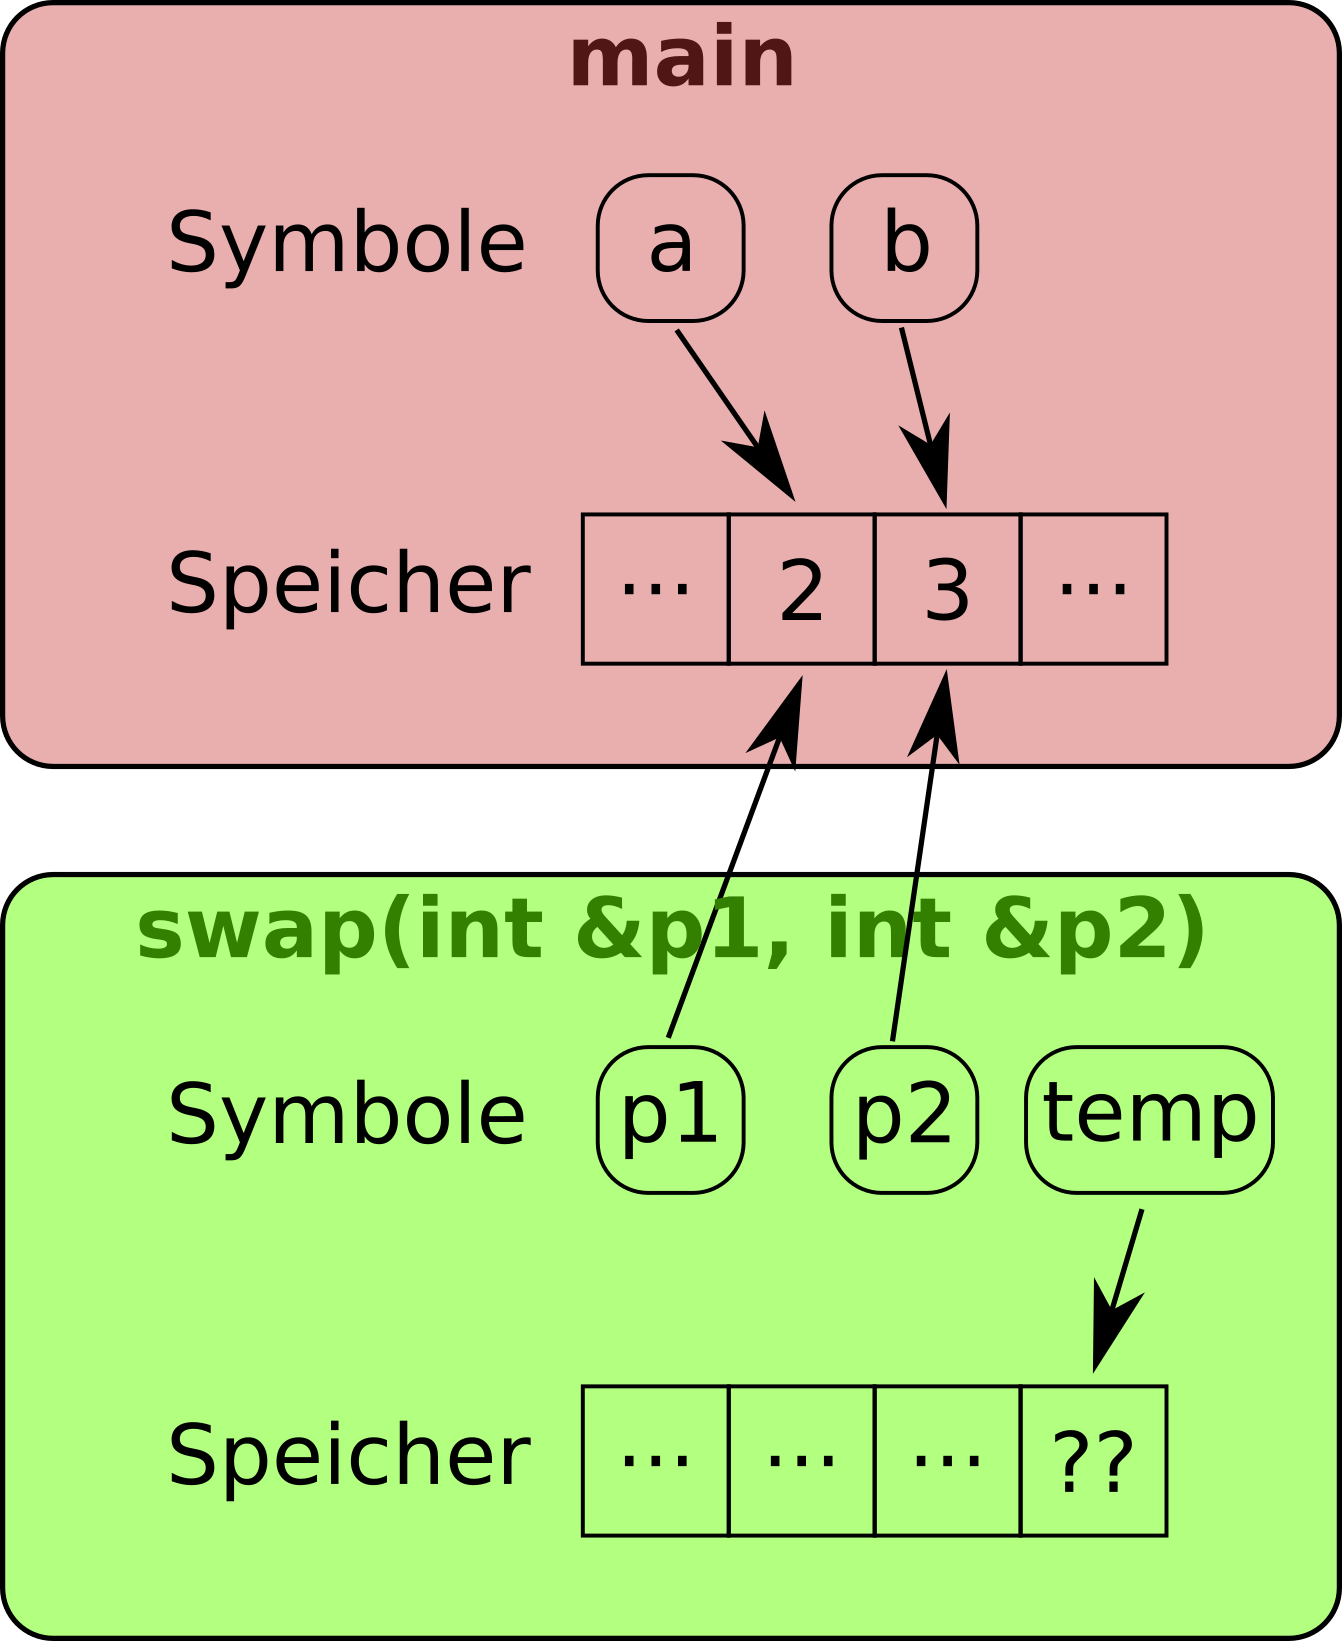
\includegraphics[width=0.6\textwidth]{img/swap_ref.png}
\end{center}
\end{frame}
\section{Casten}
\label{sec:orgff6fa73}
\begin{frame}[label={sec:orgbeb0e11},fragile]{Casten "normaler" Datentypen}
 Casten einer "normalen" Variable konvertiert (so gut wie möglich) den
Inhalt einer Variable in einen anderen Datentyp
\begin{minted}[numberblanklines=false,fontsize=\scriptsize]{c++}
int i1 = 23;
double d1 = (double)i; // Konvertiert i explizit nach double
double d2 = 23.42;
int i2 = d2; // Hier wird implizit von double nach int konvertiert
\end{minted}
\end{frame}
\section{Der Upcast}
\label{sec:org441429a}
\begin{frame}[label={sec:org52ca310}]{Upcast}
\begin{itemize}
\item Wenn sich Klassen in einer Vererbungshierarchie befinden, kann ohne
weiteres von einer abgeleiteten Klasse zu einer Basisklasse gecastet
werden
\item Das ist kein Problem, weil bei der abgeleiteten Klasse ja nur Sachen
zur Basisklasse hinzugekommen sind
\item Man bezeichnet so eine Konvertierung von einer abgeleiteten Klasse
zu einer Basisklasse als \alert{upcast} (weil man in der Klassenhierarchie
nach Oben wandert)
\item Wir werden uns solche Upcasts an Hand von impliziten casts anschauen
(also Konvertierungen die automatisch passieren)
\end{itemize}
\end{frame}
\begin{frame}[label={sec:org77db962},fragile]{Der Upcast --- Beispiel}
 \begin{minted}[numberblanklines=false,fontsize=\scriptsize]{c++}
#include <iostream>
using namespace std;

class Basis {
public:
  int a;
  void print() { cout << "Basisklasse mit Nummer " << a << endl; }
};

class Abgeleitet : public Basis {
public:
  int b;
    void print() { cout << "Abgeleitete Klasse mit Nummern " << a
			<< " und " << b << endl; }
};

int main() {
  Abgeleitet ab;
  ab.a = 42; ab.b = 23;
  ab.print(); // Abgeleitete Klasse mit Nummer 42 und 23
  Basis bc = ab;
  bc.print(); // Basisklasse mit Nummer 42
  Basis &b = ab;
  b.print(); // Basisklasse mit Nummer 42
}
\end{minted}
\end{frame}
\begin{frame}[label={sec:org8f7b0ea}]{Der Upcast --- Graphische Visualisierung}
\begin{center}
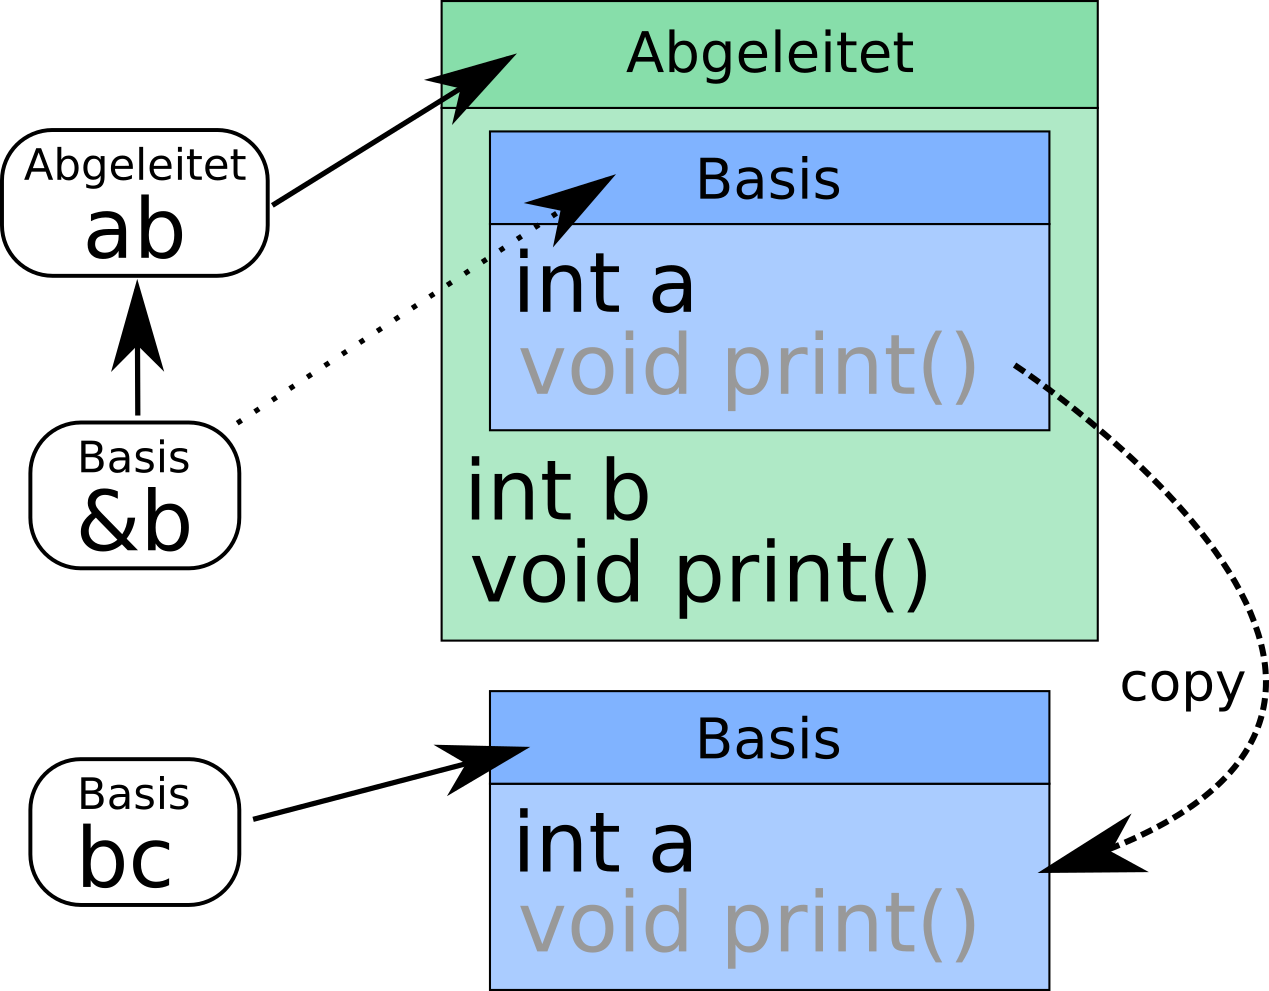
\includegraphics[width=.9\linewidth]{img/slizing_full.png}
\end{center}
\end{frame}
\begin{frame}[label={sec:org15afb5d},fragile]{Das Slicing Problem}
 \begin{itemize}
\item Aus Sicht der Referenz {\color{solarizedYellow}\verb!b!} haben wir es nun mit einer Instanz der
Klasse {\color{solarizedYellow}\verb!Basis!} zu tun.

\begin{center}
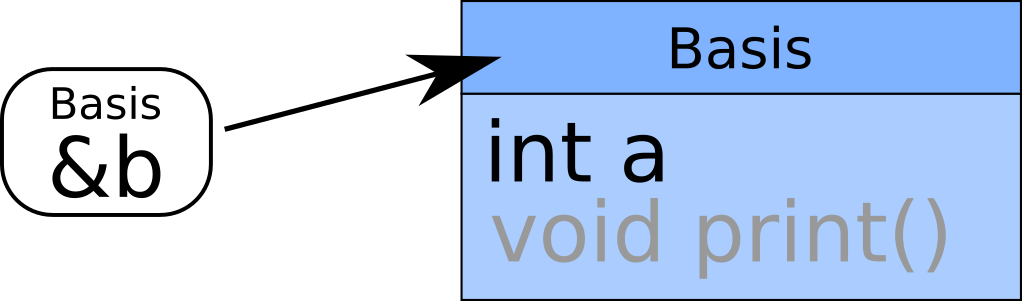
\includegraphics[width=.9\linewidth]{img/slizing_small.png}
\end{center}
\item {\color{solarizedYellow}\verb!b!} hat also "vergessen", dass es auf einen Teil einer
{\color{solarizedYellow}\verb!Abgeleitet!}-Klasse verweist
\item Beim kopieren für die Variable {\color{solarizedYellow}\verb!bc!} wurde nur der Basis-Teil kopiert
\item Man bezeichnet das als Slicing-Problem, weil Teile einer Klasse
tatsächlich, oder scheinbar abgeschnitten werden
\end{itemize}
\end{frame}
\begin{frame}[label={sec:org8b603eb}]{Der Upcast --- Was passiert}
\begin{center}
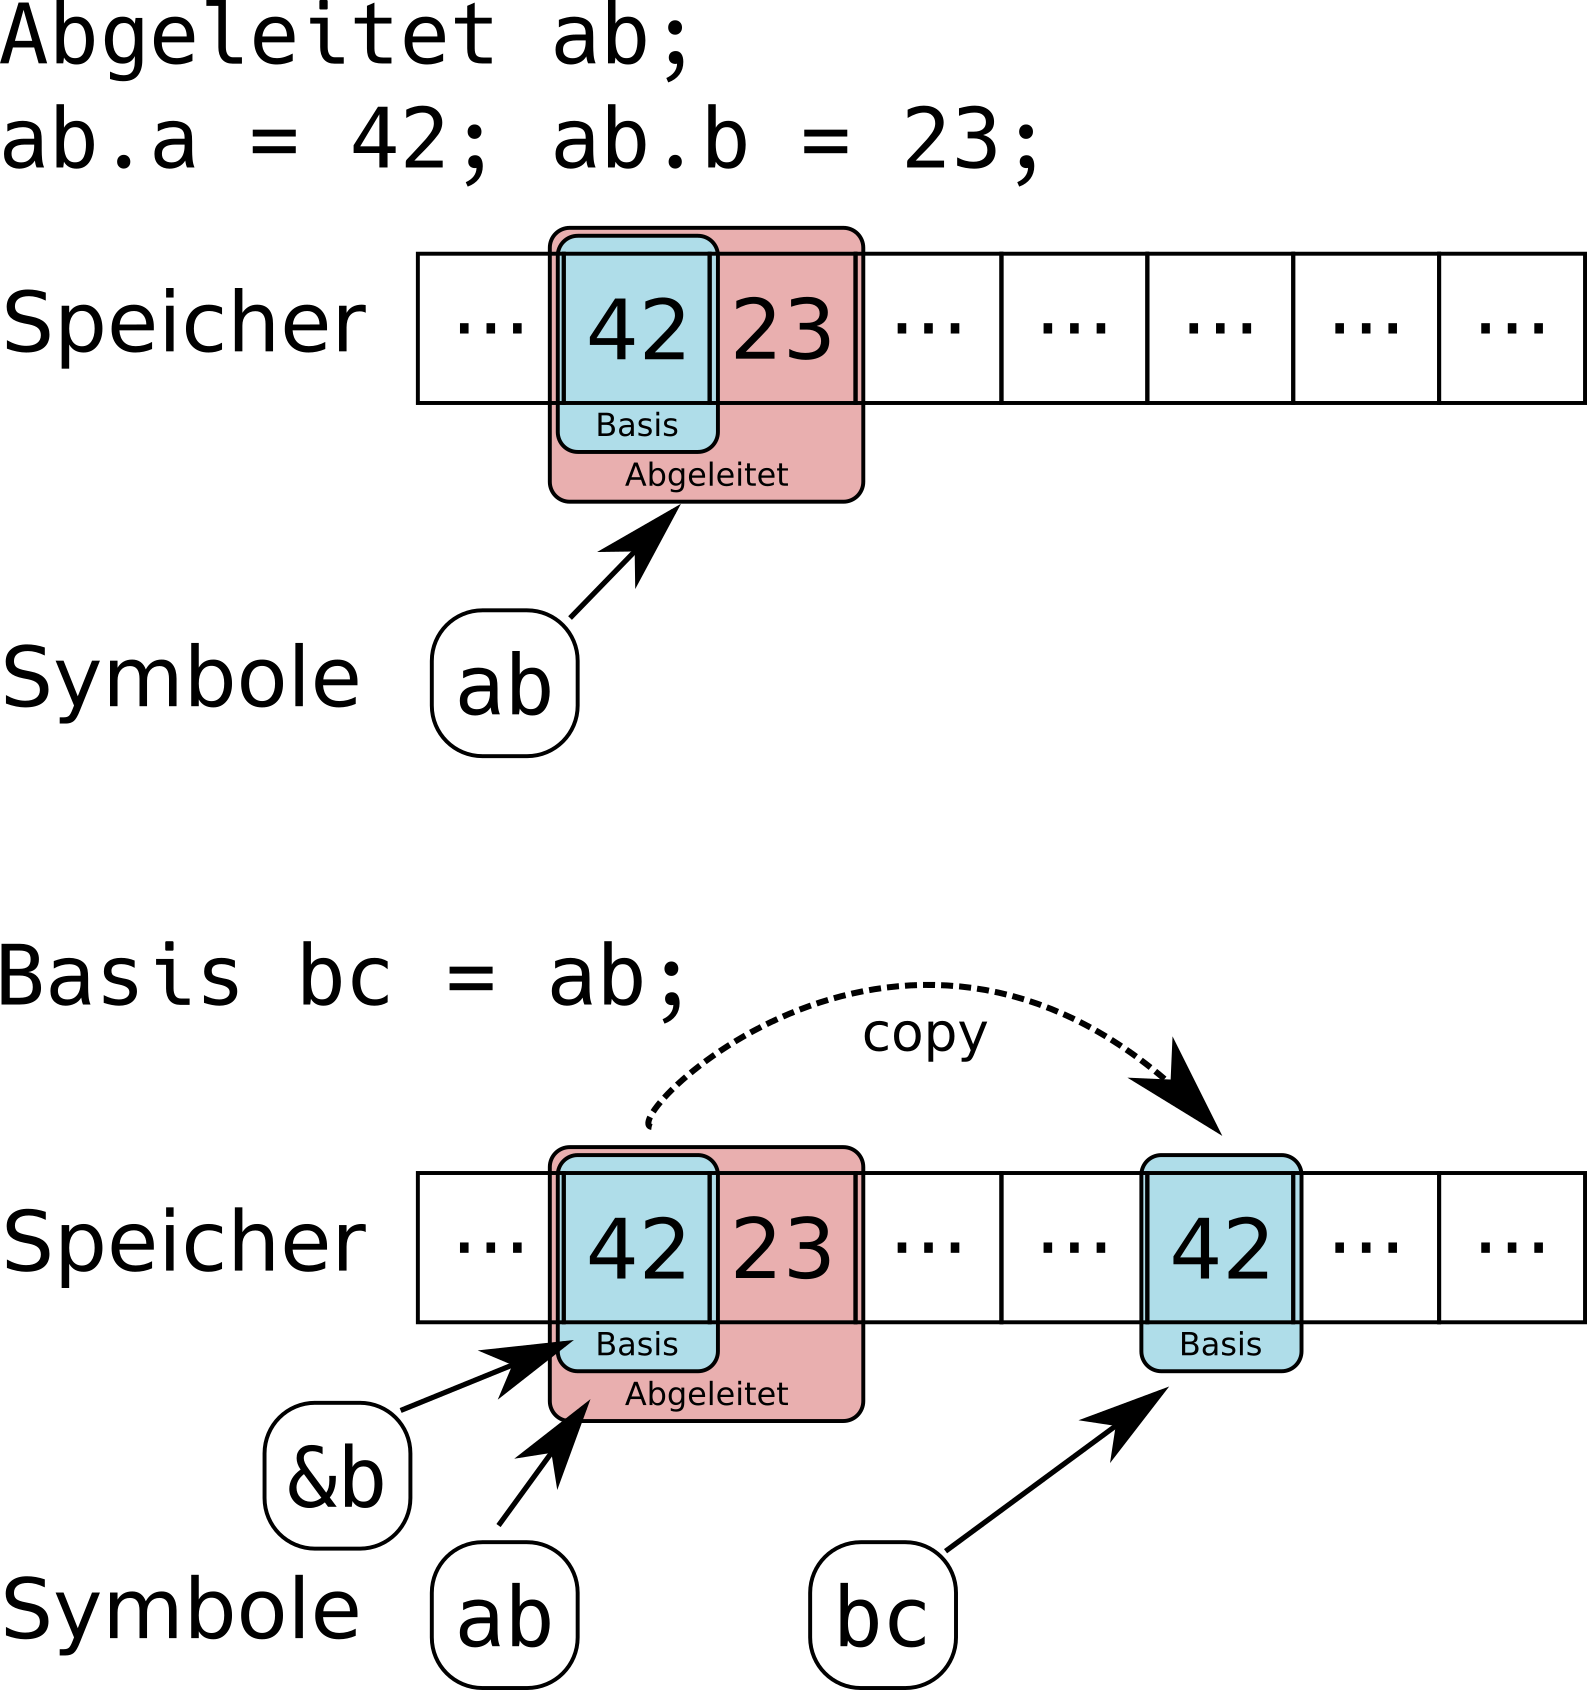
\includegraphics[width=0.65\textwidth]{img/upcast.png}
\end{center}
\end{frame}
\begin{frame}[label={sec:org0d2e6e5},fragile]{Der Upcast --- Parameter Beispiel}
 \begin{minted}[numberblanklines=false,fontsize=\scriptsize]{c++}
#include <iostream>
using namespace std;

class Basis {
public:
  int a;
  void print() { cout << "Basisklasse mit Nummer " << a << endl; }
};

class Abgeleitet : public Basis {
public:
  int b;
    void print() { cout << "Abgeleitete Klasse mit Nummern " << a
			<< " und " << b << endl; }
};

void callmyprint(Basis &b) { b.print(); }

int main() {
  Abgeleitet ab;
  ab.a = 42; ab.b = 23;
  ab.print(); // Abgeleitete Klasse mit Nummern 42 und 23
  callmyprint(ab); // Basisklasse mit Nummer 42
  // ab wird implizit in Basis konvertiert
}
\end{minted}
\end{frame}
\begin{frame}[label={sec:orgef210a4}]{Effekt eines Upcasts}
\begin{itemize}
\item Wird eine abgeleitete Klasse in den Typ einer Basisklasse
konvertiert, vergisst die Instanz was sie vorher einmal war und
verhält sich dann als wäre es schon immer eine Basisklasse gewesen
\item Dieses Verhalten bezeichnet mal als \alert{slicing} und ist oft nicht was
man will
\item Auf den nächsten Slides werden wir uns das Problem näher ansehen und
mit sogenanntem \alert{Polymorphismus} eine Lösung finden
\end{itemize}
\end{frame}
\section{Polymorphismus}
\label{sec:org0b48c44}
\begin{frame}[label={sec:orga4e1776},fragile]{Ein kleines Beispiel}
 \begin{minted}[numberblanklines=false,fontsize=\scriptsize]{c++}
#include <iostream>
using namespace std;

class Basis {
public: void print() { cout << "Hallo von der Basisklasse" << endl; }
};
class Abgeleitet1 : public Basis {
public: void print() { cout << "Hallo von der abgeleiteten Klasse 1" << endl; }
};
class Abgeleitet2 : public Basis {
public: void print() { cout << "Hallo von der abgeleiteten Klasse 2" << endl; }
};

void print_with_introduction(Basis &a) {
  cout << "Unsere Klasse möchte folgendes sagen: " << endl;
  a.print();
}

int main() {
  Basis b; Abgeleitet1 a1; Abgeleitet2 a2;

  print_with_introduction(b);
  print_with_introduction(a1);
  print_with_introduction(a2);
}
\end{minted}
\end{frame}
\begin{frame}[label={sec:orgc6baf5d},fragile]{Was ist das Problem?}
 \begin{itemize}
\item Wir hätten gerne, dass sich die Klassen mit ihren tatsächlichen
{\color{solarizedYellow}\verb!print!} Funktionen melden und nicht mit der Standardimplementierung
der Basisklasse
\item Das funktioniert aber auf Grund des Slicing-Problems nicht
\end{itemize}
\begin{block}{Lösung}
Die Lösung ist das Schlüsselwort {\color{solarizedYellow}\verb!virtual!}. Wenn in einer Basisklasse
vor einer Funktion {\color{solarizedYellow}\verb!virtual!} steht, so merkt sich die Klasse welche
Funktion einer abgeleiteten Klasse tatsächlich aufgerufen werden muss.
\end{block}
\begin{block}{Warum ist virtual nicht Standard?}
Der Aufruf einer {\color{solarizedYellow}\verb!virtual!}-Funktion ist langsamer, weil das System
zuerst nachsehen muss welche Funktion tatsächlich aufgerufen werden
muss. Zudem verbraucht eine {\color{solarizedYellow}\verb!virtual!}-Funktion Speicher in jeder
Instanz einer Klasse, weil irgendwo gespeichert werden muss welche
Funktion wirklich aufzurufen ist.
\end{block}
\end{frame}
\begin{frame}[label={sec:org15c495a},fragile]{Virtual --- Beispiel}
 \begin{minted}[numberblanklines=false,fontsize=\scriptsize]{c++}
#include <iostream>
using namespace std;

class Basis {
public: virtual void print() { cout << "Hallo von der Basisklasse" << endl; }
};
class Abgeleitet1 : public Basis {
public: void print() { cout << "Hallo von der abgeleiteten Klasse 1" << endl; }
};
class Abgeleitet2 : public Basis {
public: void print() { cout << "Hallo von der abgeleiteten Klasse 2" << endl; }
};

void print_with_introduction(Basis &a) {
  cout << "Unsere Klasse möchte folgendes sagen: " << endl;
  a.print();
}

int main() {
  Basis b; Abgeleitet1 a1; Abgeleitet2 a2;

  print_with_introduction(b);
  print_with_introduction(a1);
  print_with_introduction(a2);
}
\end{minted}
\end{frame}
\begin{frame}[label={sec:org22cb5c1}]{Wann verwendet man Polymorphismus}
\begin{itemize}
\item Man hat eine Basisklasse die ein bestimmtes Verhalten implementiert
\item Davon leitet man mehrere Klassen ab die dieses Verhalten erweitern
\item Man kann jetzt eine Funktion für die Basisklasse schreiben, und als
Parameter alle abgeleiteten Klassen verwenden, oder \ldots{}
\item wir können in einem Vektor oder in einem Array vom Typ der
Basisklasse auch alle abgeleiteten Klassen speichern (als Zeiger
oder Referenz)
\end{itemize}
\end{frame}
\begin{frame}[label={sec:orgfcbdd6b},fragile]{Beispiel --- Vektor mit Zeigern}
 \begin{minted}[numberblanklines=false,fontsize=\scriptsize]{c++}
#include <iostream>
#include <vector>
using namespace std;

class Basis {
public: virtual void print() { cout << "Hallo von der Basisklasse" << endl; }
};
class Abgeleitet : public Basis {
public: void print() { cout << "Hallo von der abgeleiteten Klasse 1" << endl; }
};

int main() {
  vector<Basis *> vec;
  Basis b1, b2;
  Abgeleitet a1, a2;
  vec.push_back(&b1);
  vec.push_back(&b2);
  vec.push_back(&a1);
  vec.push_back(&a2);

  for (auto &e : vec)
    (*e).print();
}
\end{minted}
\end{frame}
\begin{frame}[label={sec:orgb704908},fragile]{Beispiel --- Vektor mit Referenzen}
 \begin{minted}[numberblanklines=false,fontsize=\scriptsize]{c++}
#include <functional>
#include <iostream>
#include <vector>

using namespace std;

class Basis {
public:
  virtual void print() { cout << "Hallo von der Basisklasse" << endl; }
};
class Abgeleitet : public Basis {
public:
  void print() { cout << "Hallo von der abgeleiteten Klasse 1" << endl; }
};

int main() {
  vector<reference_wrapper<Basis>> vec;
  Basis b1, b2;
  Abgeleitet a1, a2;
  vec.push_back(b1); vec.push_back(b2);
  vec.push_back(a1); vec.push_back(a2);

  for (Basis &e : vec)
    e.print();
}
\end{minted}
\end{frame}
\begin{frame}[label={sec:org4401701},fragile]{Übung --- Employee und Manager}
 \footnotesize
\begin{itemize}
\item Implementieren Sie die beiden Klassen {\color{solarizedYellow}\verb!Employee!} und {\color{solarizedYellow}\verb!Manager!}
\item {\color{solarizedYellow}\verb!Employee!} ist die Basisklasse, {\color{solarizedYellow}\verb!Manager!} ist die abgeleitete
Klasse. Ein Manager ist also auch ein Angestellter
\item {\color{solarizedYellow}\verb!Employee!} hat eine Variable {\color{solarizedYellow}\verb!salary!} die speichert wie viel der
jeweilige Mitarbeiten verdient
\item {\color{solarizedYellow}\verb!Employee!} hat eine Funktion {\color{solarizedYellow}\verb!raise!} mit der man einem Mitarbeiter
eine Gehaltserhöhung geben kann. Damit der unsere Mitarbeiter nicht
zu viel verdienen, wird der maximale Gehalt auf {\color{solarizedYellow}\verb!3500!} beschränkt
\item {\color{solarizedYellow}\verb!Employee!} hat auch eine Funktion {\color{solarizedYellow}\verb!print!} die ausgibt: {\color{solarizedYellow}\verb!Der!
  \verb!Mitarbeiter hat einen Gehalt von ...!}
\item Im {\color{solarizedYellow}\verb!Manager!} wird die Funktion {\color{solarizedYellow}\verb!raise!} überladen und das Gehalt ist
nicht beschränkt
\end{itemize}
\begin{block}{Verwendung}
\begin{itemize}
\item Erzeugen Sie einen Vektor und füllen Sie ihn mit einigen {\color{solarizedYellow}\verb!Employee!}
sowie {\color{solarizedYellow}\verb!Manager!} Instanzen (entweder mit Zeigern oder Referenzen)
\item Iterieren Sie über den Vektor und rufen {\color{solarizedYellow}\verb!raise!} sowie {\color{solarizedYellow}\verb!print!} auf
und beobachten Sie das Verhalten
\end{itemize}
\end{block}
\end{frame}
\begin{frame}[label={sec:org4b285dd}]{Hinweis}
\begin{itemize}
\item \alert{Polymorphismus} ist ein weiterführendes Thema der
Objektorientierten Programmierung und uns fehlen einige Grundlagen
um das Konzept wirklich gut nützen zu können (z.B. dynamische
Speicherverwaltung)
\item Es geht in erster Linie darum, \alert{dass sie das Konzept gehört haben}
und sich zumindest ungefähr vorstellen können um was es geht
\item Sie müssen Polymorphismus im Abschlussprojekt nicht verwenden.
\end{itemize}
\end{frame}
\end{document}
